%!TEX root = paper.tex


\subsection{Installation Environment}

%{\bf Reproducibility.}
%\paragraph{Reproducibility}
Spack is intended to build a consistent HPC stack for our multi-user
environment, and reproducible builds are one of our design goals.
Experience at LLNL has shown that it is vexingly difficult to reproduce
a build manually.
%
Many packages used at LLNL have a profusion of build options, and specifying them 
correctly often requires tedious experimentation.  This is due to lack of
build standards and to the diversity of HPC environments.  
For example, in some packages that depend on the {\tt Silo} library,
the {\tt ---with-silo} parameter takes a path to {\tt Silo}'s installation prefix.
In others, it takes the {\tt include} and {\tt lib} subdirectories,
separated by a comma.
The {\tt install()} method in Spack's package files allows us to record
precise build incantations for later reuse.

%{\bf Environment isolation.}
\paragraph{Environment isolation}
In addition to command-line issues, we
frequently encounter errors due to inconsistencies between the environment of
the package installer and the package user.
%
For example, there are two versions of the {\tt libelf} library used by
LLNL performance tools. One is distributed with RedHat Linux, while another
publicly available version has the same API but an incompatible ABI.
Failure to specify the right version at build time has caused many
inexplicable crashes.
%
Spack manages the build environment by running the {\tt install} invocation
in a new process.  It helps packages find dependencies 
correctly, by setting
{\tt PATH}, {\tt PKG\_CONFIG\_PATH}, {\tt CMAKE\_PREFIX\_PATH}, and
{\tt LD\_LIBRARY\_PATH} to include the dependencies of the current build.
These variables are commonly used by build systems to locate dependencies,
and setting them helps to ensure that incorrect libraries are detected.
The isolated build environment also gives package authors 
free reign to set build-specific environment variables without interfering
with other packages.


%{\bf Compiler wrappers and RPATHs.}
\paragraph{Compiler wrappers and RPATHs}
Finding compilers at build time is not the only obstacle to reproducible
behavior.  As mentioned in Section~\ref{sec:motivation}, it is also important
for binaries to be able to find dependency libraries at {\it runtime}.
One of the most frequent user errors at LC is improper library configuration.
Users frequently do not know what libraries a package was built with, and 
it is difficult for them to construct a suitable {\tt LD\_LIBRARY\_PATH} for
a package that was built by someone else.  Because of frequent support calls,
we typically add {\tt RPATHs} to public software installations, so that paths
to dependencies are embedded in binaries and so that users do not have to know
this information to run installed software correctly.

Spack manages {\tt RPATH} settings and other build policies with
{\it compiler wrappers}. 
In each isolated {\tt install} environment, Spack sets the standard 
environment variables
{\tt CC}, {\tt CXX}, {\tt F77}, and {\tt FC} to point to its own compiler
wrapper scripts.  These variables are used by most build systems to select
C, C++, and Fortran compilers, so they are generally picked up 
automatically\footnote{If builds do not respect {\tt CC}, {\tt CXX}, etc.,
wrappers can typically be added as arguments or inserted into Makefiles
by {\tt install}.}.
When run, the wrappers insert include ({\tt -I}), library ({\tt -L}), and 
{\tt RPATH} ({\tt -Wl,-rpath} or similar) flags into the argument list.
These point to the {\tt include} and {\tt lib} directories of dependency
library installations, where needed headers and libraries are typically located.
After the modified argument list is constructed, the wrappers delegate it
to the real compiler to execute.

Spack's compiler wrappers have a number of useful effects.  First, they allow
Spack to transparently parametrize the compiler for most builds and for
Spack users to easily request a build with a new compiler swapped in.
Second, they enforce the use of {\tt RPATHs} in
installed binaries.  This causes applications built by Spack to run correctly
{\it regardless of the environment}.  Third, because compiler wrappers add 
header and library search paths for dependencies, header and library detection
tests run by most build systems succeed automatically, {\it without}
the need to use special arguments for nonstandard locations.  {\tt configure}
commands in Spack's {\tt install} function can have fewer arguments, and can
be written as they would be for system installs.  This reduces complexity
for package maintainers and enforces consistent, reproducible
build policies across packages.  Finally, because Spack has control over the 
wrappers, package authors can programmatically filter the compiler flags
used by software build systems, a useful last resort when porting to
bleeding-edge platforms or new, esoteric compilers.

\subsubsection{Environment Module Integration}
\label{sec:envmodule}
In addition to build-time environments, Spack can also assist in create run-time
environments.  A package may need environment variables like {\tt PATH}, 
{\tt LD_LIBRARY_PATH}, or {\tt MANPATH} set before they can be used.  Some users
may prefer to manually point environment variables and paths at packages, and 
Section~\ref{sec:package-views} discusses how Spack can assist those users.  
As discussed in Section~\ref{sec:motivation}, many sites rely on environment 
modules to set their runtime environment.  Spack can automatically create 
dotkit~\cite{dotkit} and Module configuration files for its packages, allowing 
users to setup their runtime environment using familiar systems.  

Future versions of Spack may also allow the creation of Lmod~\cite{mclay:lmod} 
module files.  Lmod allows users to load packages using a heirarchy of module 
load operations.  For example, a user might load a {\tt gcc} module and a 
{\tt mvapich2} module, and a subsequent load of the {\tt MPILeaks} package would 
load the appropriate version for that compiler and MPI implementation.  Spack 
understands where packages would fit in the Lmod hierarchy, allowing it to create 
Lmod module files.  

\begin{figure}\centering
	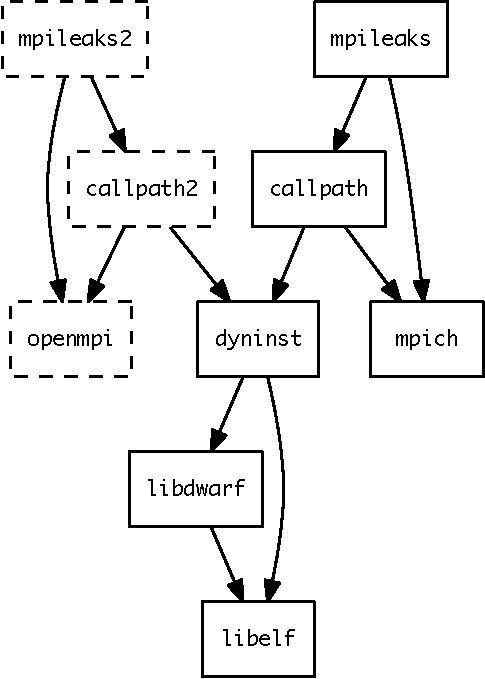
\includegraphics[width=.6\linewidth]{specs/rpaths.pdf}
	\newline
	\verb|spack install mpileaks ^mpich|\newline
	\verb|spack install mpileaks ^openmpi|
	\caption{
		Installing {\tt mpileaks} with MPICH (solid), then with OpenMPI (dashed).  The {\tt dyninst} subtree is
		reused, but {\tt mpileaks} and {\tt callpath} must be rebuilt.
	}
\end{figure}

